\chapter{The effects of radiation in silicon detectors}% No definitivo
\label{chap:rad}
% I haven't talked about leakage current and I most certainly should

When a particle goes through a silicon detector, it can loose energy via ionisation, which is a reversible process because the electrons extracted from the atoms will end up recombining. The particle can also lose energy via non-ionising interactions, where the particle interacts with the Silicon atoms or with the dopant atoms. The effect is detrimental for the detector and leads to a reduction of the collected charge, amongst other macroscopical effects. It is important to understand these changes and have a parametrisation of the degradation. Understanding these defects is fundamental for designing radiation-hard detectors.

In this chapter we summarise the most important mechanisms of radiation damage. One of the key points of the project was to implement radiation damage on the TRACS simulator.


\section{Damaging the lattice}% No definitivo

\begin{figure}[H]
	\centering
	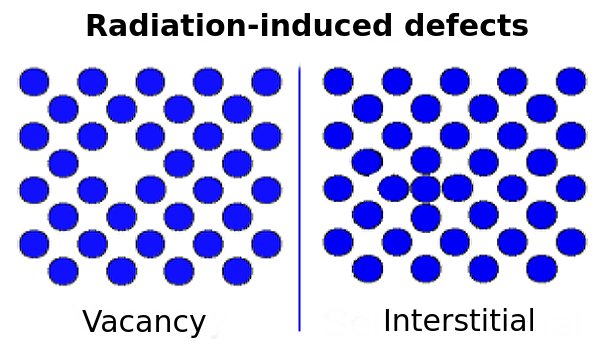
\includegraphics[width=0.8\textwidth]{chap3_defects.png}
	\caption{Interstitial (right) and Vacancy (left) lattice defects are illustrated here. This defects are be created inside silicon detectors after irradiation.}
	\label{fig:IV}
\end{figure}

When a particle transversing the silicon detector undergoes a non-ionising interaction one or more atoms get knocked-out from their equilibrium position in the lattice, disrupting the ordered structure of silicon. If the atom does not return to the equilibrium position, and Interstitial-Vacancy (I-V) defect is created. The term Interstitial refers to the knocked-off atom misplaced in the lattice and the Vacancy refers to the empty place that it leaves behind as shown in Figure \ref{fig:IV}. This type of defect alters the ordered structure of the lattice and creates new energy. The mechanisms by which the I-V defects degrade the performance of the detector and its practical consequences will be discussed in the next sections.

%When a particle goes through a silicon detector it can ionise the material and move electrons out of the valence band into the conduction band generating an electrical signal than be read, as we have previously discussed. Another possibility is that the particle knocks off one or more of the silicon atoms that compose the lattice. In this case the atom might return to its original position if the momentum transfer is small dissipating the extra energy via thermal vibrations or it might get knock off completely from its original position. In the latter case the lattice presents now a defect that will influence its properties. For this section we will only focus on the types of defects and their evolution, leaving their effects to the next two sections. 

An inpinning particle can create more than one I-V defects provided it has enough energy. The second I-V defects can be created directly by the particle or by the recoil atom if enough energy was transferred to it. The size and clustering of the defects depends on the energy and type of radiation. 

%During the radiation process, either in a controlled environment for research purposes or as a side effect of particle detection, various types of particles with different energies might transverse the silicon detector might have different damaging effects in the silicon lattice. When an inpinning particle knock off an atom the result is an interstitial-vacancy pair. The knocked-off atoms sitting in a different position between other silicon atoms is what we call interstitial defect and the lack of such atom on its original position is called vacancy. Depending on the inpinning particle type and the energy transferred to the recoil atom more than vacancy-interstitial defects might be created after the first impact. The size and clustering of these defects depends strongly on the energy of the particles and also on their characteristics. 

For example, according to \cite{MMoll}, photons with up to 1 MeV energies will create only point defects with no clustering effects. Electrons can create both point defects and clusters of defects, with clusters only occurring for electron energies above 8 MeV. Neutrons will create mainly clusters starting at energies as low as 35keV. 

Typically the NIEL (Non-Ionising Energy Loss) hypothesis is used to characterise the radiation damage caused by any type of particle. The NIEL hypothesis states that the damage produced by radiation of any kind of particle is proportional to the damage produced by 1 MeV neutrons. Therefore fluence of any type of radiation is rescaled to the equivalent fluence of 1MeV neutrons. %the standard unit of measuring the radiation that a silicon detector has undergone is the neutron equivalent (neq).

The I-V defects induced by radiation are not necessarily static defects and their size and configuration may vary in time. The damage due to radiation evolves with time. For instance, the depletion voltage first decreases with time at a fixed temperature (so-called beneficial annealing) to increase linearly afterwards (long term annealing). The evolution speed depends heavily on temperature. Evolution achieved in around 21h at 60C can be slowed down to about 500 years just by cooling down the irradiated detector to -10C. 

The standard procedure followed by researchers includes an intentional annealing phase so that all irradiated detectors have undergone similar damage evolution. The annealing time depends on the transport and irradiation conditions. Irradiated sensors are stored in cold environments such as fridges.

%Another important aspect of radiation damage and radiation-induced defects is their evolution in time. It has been shown that the effects of radiation on silicon detector evolve with time even after the irradiation has been stopped. Studies on annealing of irradiated silicon detectors show that typically there is a beneficial evolution right after the irradiation process in which the silicon damage becomes smaller. After this stage annealing increases the damage on irradiated silicon detectors with time reaching levels well over the initial state right after irradiation. This process can be slowed down by lowering the temperature of the detector. Evolution achieved in around 21h at 60C can be slowed down to about 500 years just by cooling down the irradiated detector to -10C. It is for this reason that silicon detectors are usually annealed for a short period of time after irradiation, and the stored at low temperatures for transport and experimental measurements.

\section{Trapping effects} % No definitivo
\label{sec:trapEfect}

%Defects in the silicon lattice have no effect in the generation of $e-h$ pairs but do have an effect in their drift and collection. This is due to the defects introducing what are called $deep$ levels. Such deep levels lie in the gap between the conduction and valence bands but much further from them than the shallow levels introduced by impurities as explained in section [SECTION].

%Deep levels can be filled by electrons or holes depending on their proximity to the valence or conduction band respectively. The main effect of these deep levels is trapping charge carriers for a large amount of time compared with typical collection times in non-irradiated silicon detectors. The trapping of the charge carriers modifies that distribution of electrons and holes inside the detector which in turn can significantly modify the space charge distribution inside the depleted region of the detector. The drift of both charge carriers is also affected by these changes as we will see in detail later. In special cases the effect can be so strong that type inversion might occur. When this happens the previously $p$ doped part of the silicon detector becomes effectively $n$ doped. This effect of type inversion does not happen in initially $n$ doped silicon.

%If one looks at the radiation-generated deep levels, they can hold charge carriers for long times before realising it. This process disrupts temporarily the $N_{eff}$ inside the silicon detector. If the trapping-releasing cycle happens with enough frequency (as it is the case under most circumstances) then the \neff can be thought of being permanently modified by the charges trapped in the deep levels. As opposed to the unirradiated case, now the \neff is not a constant but has a different shape. Since the \neff is one of the most important things in signal development inside the silicon detector, it is of great importance that its modification due to radiation damage are well known.

%Being, as it still is, a body of great debate, \neff parametrisation has yet to find a definitive answer that can be successfully applied in all cases. For now we will focus on mainly two parametrisation of said variable for those two are the most succesful and widely accepted, but it should be noted, again, that \neff evolution with radiation damage is not fully understood at the time of writing this work. First of the parametrisation was introduced in 2002 and devised the \neff inside the detector to change shape from constant to linear with depth. In this model the already present electric field inside the detector would force influence charge carriers to move to both ends of the detector (depending on the charge sign) creating an excess of positive charges on one side and a excess of negative ones on the other compared to the non-irradiated state. The resulting \neff is a straight line that gives rise to a parabolic electric field that will change the shape of the collected signal in accordance to experimental results.

%The second mayor parametrisation that should also be considered in the frame of this project is a variation on the basic fundamentals of the linear model. This next model was proposed more recently by G.Kramberger and states that the shape of \neff after irradiation can be parametrised in some cases as being constant in three separated regions. As it can be seen in Figure FIGURE\_3ZONE\_NEFF each of the three parts of the \neff would be constant generating a linear electric field with three different slopes resembling the shape of the aforementioned parabola that is observed experimentally.

The defects induced by radiation only affect the drift and collection of the $e-h$ pairs. The I-V defects create the so called $deep-levels$ that can trap and hold charge carriers for times longer than the typical collection times in silicon detectors. The result is a net loss in charge collection efficiency as well as a modified \neff profile.

\begin{figure}[H]
	\centering
	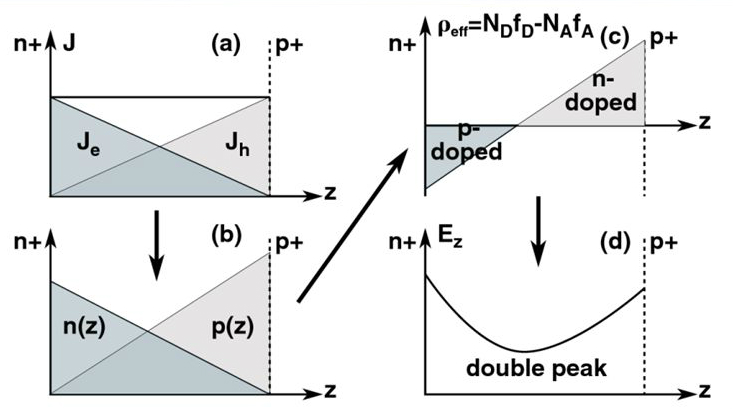
\includegraphics[width=0.8\textwidth]{chap3_erem.jpg}
	\caption{Interstitial (right) and Vacancy (left) lattice defects are illustrated here. This defects are be created inside silicon detectors after they have been irradiated.}
	\label{fig:Eremin}
\end{figure}

To explain why the \neff gets modified after irradiation, we will follow the argument presented by V.Eremin\cite{Eremin}. The current density of $e$ or $h$ ($j_i(z)$), in a fully depleted silicon detector, is not a constant but has a linear dependence with thickness ($z$), as shown  in figure \ref{fig:Eremin}\emph{a}. The concentration of carriers ($n_i(z)$) is proportional to the current $j_i(z)$, so $n_i(z)$ is also linear with $z$. After enough radiation the defects and their correspondent deep levels can be considered uniformly distributed throughout the detector. The amount of carriers trapped can be considered proportional to their concentration. Taking the charge sign into account the end result is a linear dependence of space charge distribution with $z$ (Figure \ref{fig:Eremin}\emph{b}. For a more complete description of this argumentation and its validity the reader is referred to the bibliography.


% Consecuences of a modified Neff (leakage current, higher Vdep, type inversion, DP & DJ)

One of the consequences of having a non-constant \neff configuration is that the resulting electric field inside the detector gets modified. In the linear case mentioned above a parabolic electric field appears (see Figure \ref{fig:Eremin}\emph{c}) giving rise to a characteristic \emph{double peak} (DP) shape of the transient waveforms. Another consequence of not having a constant \neff is the appearance of a second $p-n$ junction at the end of the detector creating the double junction (DJ) effect. The apparition of the DJ means that in a detector not fully depleted both ends remain sensitive to radiation.

%Other effects of the modified \neff of lesser importance for this project are the increase in leakage current, a higher \vias needed for depleting the full detector volumen, and more exotic processes such as type inversion. % Deberia hablar algo mas de type inversion? decir lo que es?

% EXPLAIN WHY IT MIGHT NOT BE LINEAR but something more exotic (link with TRACS capabilities)

So far it has only been considered that the modification of the \neff due to radiation-induced defects gives rise to a linear \neff inside the detector. However, this might not be always the case, as it has been proposed in more recent publications\cite{KramVertex}. Analysis performed using edge-TCT techniques suggest that the \neff configuration might have three different regions in which its value remains constant. This parametrisation will be referred to as \emph{triconstant} and can also explain the DJ and DP effects seen experimentally. As it will be explained in detail later, both linear and triconstant parametrisations have been implemented into TRACS as well as a third parametrisation consisting of three linear regions.  

On top of the \neff modification, the deep levels induced by radiation have also an impact on signal collected from the detector. When charge carriers drift through the irradiated volume they may get trapped in a radiation-induced defect and remain there for as long as several miliseconds. This is much longer than the collection time (of the order of tens of nanoseconds) so they are effectively lost. As a result, the waveform shape gets distorted (as it will be explained in the following section) and the charge collected decreases worsening the performance of the detector.

\section{Signal degradation} % No definitivo
\label{sec:signalDeg}

%After taking a look at the effects that radiation has on silicon it is important to understand how radiations changes the read-out signal, since that is what will be measured in the laboratory. As we have already mentioned the main effect of radiation damage from a practical point of view is the creation of deep levels inside the band gap that act as trapping centers for the charge carriers moving inside the silicon bulk. For the sake of simplicity and ease of explanation when explanation when talking about the implementation of radiation damage in the software TRACS, we will treat \neff deformation as a different effect. This is very practical as it helps understand dynamical and static effects separately. 

%The effect that deep levels have in the signal is the trapping of the charge carriers creating a loss in charge collection efficiency. Because collection times in silicon detectors are of the order of tens of nanoseconds whilst the trapping times are typically of the order of milliseconds, the trapped carriers will never be released in time to be collected and are effectively lost. The process of trapping is a statistical one with the probability of one charge carrier to be trapped after a drifting inside the silicon for a time $t$ being  \[FORMULA FOR TRAPPING PROBS\] where $\tau$ (trapping time) is an experimentally determined parameter that shows how likely it is for a carrier to get trapped, in a very similar law as that governing the natural decay of radioactive materials. For a big enough number of carriers drifting in silicon, the effective result in the signal generated is an exponential decrease over time in the collected signal with respect to the unirradiated case. 

%On the other hand the \neff modification due to radiation has no effect on the total collected charge, but on the shape of the collected signal as well as in the collection time. As discussed before the intensity recorded is proportional to the electric field in which the carriers are drifting. Since the electric field is obtained by integrating the \neff, this field is now modified by radiation and yields different waveforms when measured in the lab. Since velocity is different from the non-irradiated case, collection times are modified becoming larger after irradiation in most cases due to lower electric field modulus in the middle of the bulk of silicon. 

%Both effects combined yield the typical $double peak$ shape obtained when subjecting the irradiated detectors to the TCT analysis that are normally performed in the lab. This shape combines the double peak feature of the electric field with the exponential dampening of the electrical charge collected. This kind of measurements and analysis are very useful in studying the charateristics of irradiated silicon detectors including determination of trapping times, \neff profile and charge collection efficiency, as it will be shown in the following chapter.

The effects of radiation in detector performance can be observed both in terms of the total collected charge and the shape of the transient waveforms. The modified \neff distribution inside the detector has an effect on the shape of the waveforms while the effects of trapping centers can be seen both in the waveforms and in the total collected charge.

It has been explained in section \ref{sec:Ramo} that the  $ I (t) $ profile of the collected signal from the detector depends on the $\overrightarrow E $ inside of it. It then follows that a modified \neff  (and consequently a modified  $\overrightarrow E$ ) will have an effect in the collected signal and might show a double peak (DP) due to the previously mentioned DJ effect. The collection time might also be affected for the same reason.

For the trapping effects, the probability that a carrier drifting inside the silicon gets trapped in the radiation-induced deep levels after a time $dt$ is

\[p_{trap} = 1/\lambda \cdot dt\] % Need to check bibliography

with $\lambda$ the effective carrier trapping distance that can be different for electrons and holes. We will use $\tau \approx \frac{\lambda}{v_{th}}$ with $\tau$ being the trapping time and $v_{th}$ the thermal velocity of the carrier and can be used in most situations\cite{Kramberger} since $v_{th} > v_{drift}$. The $\tau$ is an experimentally determined parameter that is usually taken to be constant or dependant on the electric field and type of carrier.For the rest of the report we will consider $\tau$ to be a constant except otherwise stated. This allows to write the number of non trapped carriers $N$ after drifting in the detector for a time $\Delta t$ as

\[N = N_0 \cdot \exp{\big(\frac{-\Delta t}{\tau}} \big)\]

where $N_0 = N(\Delta t = 0)$ the initial number of carriers generated in the detector. Since the intensity is the sum of every carrier's contribution, if we assume that every carrier contributes equally to the total current the previous equation can be re-written as

\begin{equation}
	I(t) = I_0(t) \cdot \exp{\big(\frac{-\Delta t}{\tau}\big)}
 \label{eq:trapCurr}
\end{equation}

where $ I_{0}(t)$ is the total current that would be read if there were no trapped carriers. \textbf{comento algo sobre la aproximacion? por ejemplo su validez?}

\textbf{\emph{Duda}}
(opcion 1)>>>>>>>>>>>>>>>>>>>>>>>>>>>
It might not appear to the reader why it is interesting to consider the no-trapping $I_0(t)$ on an irradiated detector with a modified \neff, but the reason will become more aparent when the implementation of radiation damage is explained. 

Opcion 2>>>>>>>>>>>>>>>>>>>>>>>>>>

This last equation has little interest from a experimental point of view but it will help to understand the implementation of trapping effects in TRACS. 

Fin opciones<<<<<<<<<<<<<<<<<<<<<<<<<<

In summary, the net result of trapping centres is to reduce the charge collected; the effect can also be seen in the transients waveform.

